%% This is an example first chapter.  You should put chapter/appendix that you
%% write into a separate file, and add a line \include{yourfilename} to
%% main.tex, where `yourfilename.tex' is the name of the chapter/appendix file.
%% You can process specific files by typing their names in at the 
%% \files=
%% prompt when you run the file main.tex through LaTeX.
\chapter{Design and Implementation}

This chapter of the study deals with the design and the implementation of the system being proposed to store disaster-related information. Here, we will look into the specific technologies used to construct the system. This system is intentionally designed to be modular so that specific technologies used can interchanged to provide improvements to the system while also making it possible to adapt the system to different types of use cases.

\begin{figure}[ht!]
	\centering
	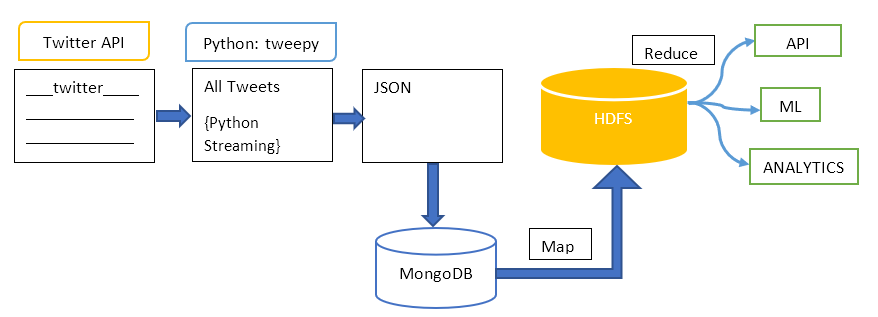
\includegraphics[width=150mm]{DesignDiagram.png}
	\caption{Disaster Management Information System design. \label{overflow}}
\end{figure}

The flow of the Disaster Management Information System design is shown in Figure 3-1. Here the Twitter Streaming API provided by Twitter is incorporated in to the system by using tweepy, a python library, to extract the disaster related data. The Streaming API provides a JSON output which is stored into MongoDB. The output of the MongoDB is parsed using a cognitive filtering system to filter out the irrelevant data and then sent to Hadoop mapper to store all the relevant information in the HDFS data store. Hadoop reduce is used to structure the relevant information and provide it to the end user.

\section{Twitter}

\subsection{Twitter API}\label{ch1:opts}

Twitter as a platform has a lot of users and it generates a lot of data that can be used for analysis. Data can include user tweets, user profiles, user followers, user status, what's trending, etc. This data can be extracted using Twitter Application Programming Interface(API). There are three methods to get this data: the REST API, the search API, and the Streaming API. The Search API is retrospective and allows to search old tweets [with severe limitations], the REST API allows you to collect user profiles, and followers, and the Streaming API collects tweets in real time as they happen. As this study concerns with the real-time analysis of the data, it is important to highlight the fact that the Streaming API is most suited for those needs.

Using the Twitter API requires a few steps:

\begin{enumerate}
  \item Authenticate with OAuth
  \item Make API call
  \item Receive JSON file back
  \item Interpret JSON file
\end{enumerate}

\subsection{Authenticate with OAuth}

OAuth is an open standard for access delegation, commonly used as a way for Internet users to grant websites or applications access to their information on other websites but without giving them the passwords \cite{gordonunderstanding}. Authentication with OAuth on Twitter requires you to get keys from the Twitter developers site using a Twitter developer account. There are four keys (Consumer Key, Consumer Secret Key, Access Token, and Secret Token) that are required to access the API and need to be used during a handshake, once authenticated the program can make API calls.

% This is an example of how you would use tgrind to include an example
% of source code; it is commented out in this template since the code
% example file does not exist.  To use it, you need to remove the '%' on the
% beginning of the line, and insert your own information in the call.
%
%\tagrind[htbp]{code/pmn.s.tex}{Post Multiply Normalization}{opt:pmn}

\subsection{Make API call:}

When making an API call to twitter it has parameters incorporated into the URL, the wrapper looks like this:

\hfill

\url{https://stream.twitter.com/1.1/statuses/filter.json?track=twitter}

\hfill

This call is being done through the streaming API, where it is asking to connect to Twitter and once connection is established it will track the keyword 'twitter'. To track specific information,  keywords can be listed and if done carefully it can filter a lot data at an early stage that is irrelevant in this research. For example, keywords such as 'hurricane', 'flood', 'epidemic', etc., can be listed to stream tweets containing these words.

Using  python library called tweepy the working of an API call is abstracted from the user, nevertheless understanding the working of making a Twitter API call is necessary to extract the relevant data.

% This is an example of how you would use tgrind to include an example
% of source code; it is commented out in this template since the code
% example file does not exist.  To use it, you need to remove the '%' on the
% beginning of the line, and insert your own information in the call.
%
%\tgrind[htbp]{code/be.s.tex}{Block Exponent}{opt:be}

\subsection{Receive JSON file back:}

JavaScript Object Notation (JSON) is an open standard file format that has data formatted as attribute-value pairs. The format is language independent and is commonly used for asynchronous browser-server communication for a data request.

JSON files is also the data structure that Twitter returns when an API call is made. The amount of data returned depends on how the keywords are defined, but is usually rather comprehensive and needs to be parsed.

\subsection{Interpret JSON file:}

JSON file can be stored as raw file or can be stored using a SQL/NoSQL database. Since the data received is unstructured the most logical way to store the data is using a NoSQL database. In this study MongoDB is used to store the tweets we receive and parse through. Next, queries are run based on the keywords that are needed to select information.

\section{Python:}

While there are many different programming languages that can be used to interface with the API, the flexibility and huge community support behind python as well as its relevance in data science makes python the ideal choice in this research. Python has many libraries that has different use cases, here tweepy is used to stream the disaster-related data from twitter.

\section{Tweepy:}

Python is a versatile language with adaptability to various use cases. These are done by extending the language by using libraries which are community created. One of these libraries is tweepy. Tweepy is open-sourced, hosted on GitHub and enables Python to communicate with Twitter platform and use its API \cite{tweepypython}. This makes it easier to access the platform to collect and monitor tweets for analysis.

\subsection{Using tweepy:}

Command to install the tweepy library:

\hfill

\begin{lstlisting}
\$ pip install tweepy
\end{lstlisting}

Tweepy supports OAuth authentication. Authentication is handled by the \\ tweepy.AuthHandler class \cite{tweepyauth}.
A consumer token and a secret key is needed to connect with the Twitter stream API, this uses the keys that were generated after a Twitter developer account was created.

These keys are a pair of private and public (secret and non-secret) keys and used to maintain security. The consumer key pair authorizes the program to use the Twitter API, and the access token essentially signs the application into specific Twitter user account. This framework makes more sense in the context of third party Twitter developers like TweetDeck where the application is making API calls but it needs access to each user's personal data to write tweets, access their time-lines, etc. \cite{collectingtwitter}.

The tweepy library can be imported as shown:

\begin{description}
\item[$\bullet$]from tweepy import Stream

\item[$\bullet$]from tweepy import OAuthHandler

\item[$\bullet$]from tweepy.streaming import StreamListener
\end{description}

The above tweepy class imports will be used to construct the stream listener.


\section{Diving into the code:}

This section helps to describe how the information is stored as a flat file and the advantages of storing the information into a NoSQL data store like MongoDB. Here, the tweepy library is shown using the Streaming API to store information.

\subsection{Importing the modules:}

\begin{figure}[ht!]
	\centering
	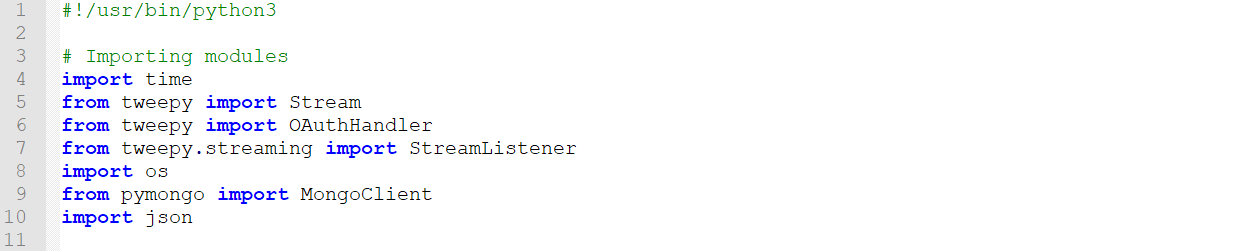
\includegraphics[width=150mm]{code11.png}
	\caption{Importing libraries. \label{overflow}}
\end{figure}

As shown in Figure 3-2, apart from the three tweepy class imports used to construct the stream listener, the time library is used to create a time-out feature for the script, and the os library is used to set the working directory.

\subsection{Setting the Variables:}

\begin{figure}[ht!]
	\centering
	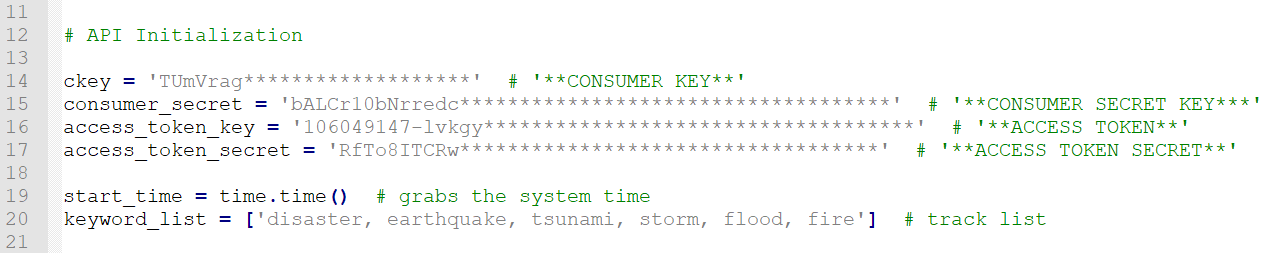
\includegraphics[width=150mm]{code21.png}
	\caption{Setting tokens. \label{overflow}}
\end{figure}

As shown in Figure 3-3, the variables have to be set, which is then used in the stream listener by being fed into the tweepy objects. Here, we set the different token keys generated by signing up for the Twitter API. These keys help to provide access without twitter divulging its authentication tokens.

\subsection{Using and Modifying the Tweepy Classes:}

The code shown in Figure 3-4 does the following:

\begin{figure}[ht!]
	\centering
	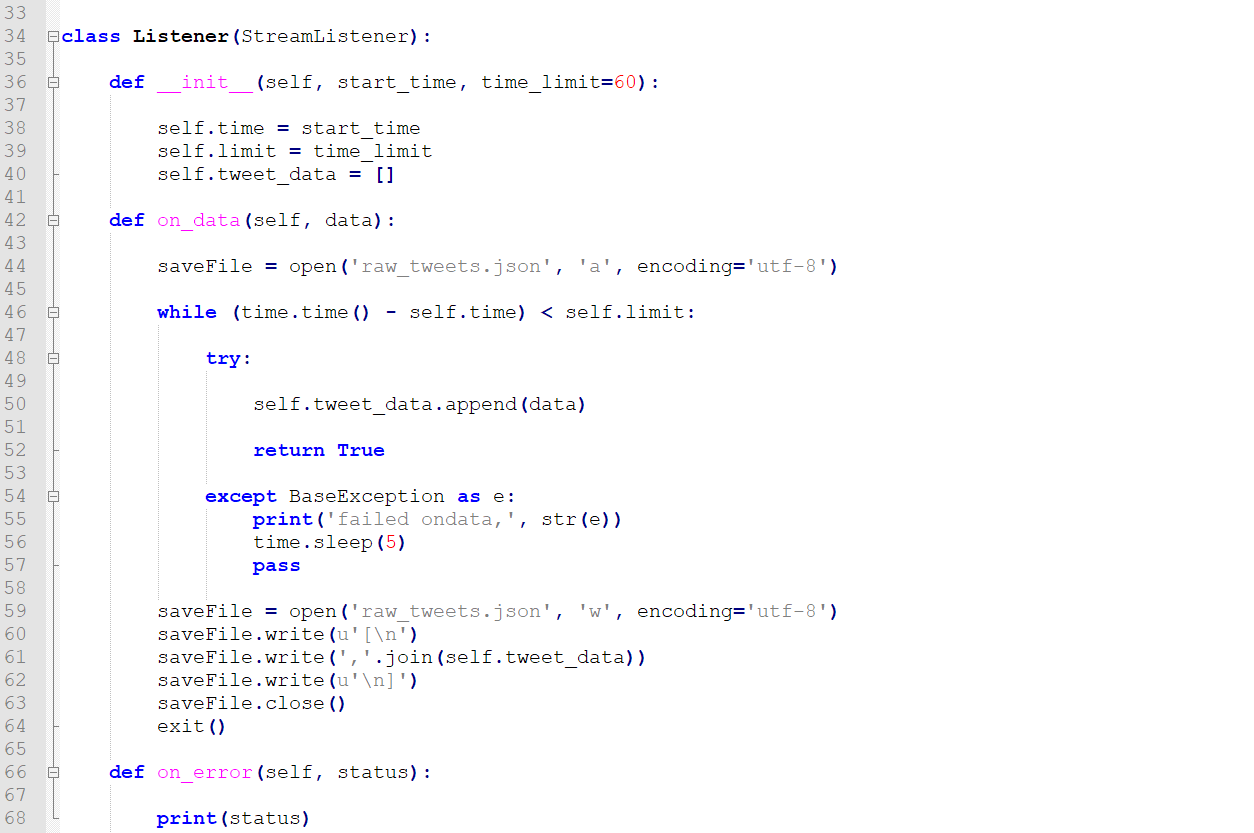
\includegraphics[width=200mm]{code31.png}
	\caption{Stream listener. \label{overflow}}
\end{figure}

\begin{description}
	
\item[$\bullet$]Creates an OAuthHandler instance to handle OAuth credentials.

\item[$\bullet$]Creates a listener instance with a start time and time limit parameters passed to it.

\item[$\bullet$]Creates an StreamListener instance with the OAuthHandler instance and the listener instance.
\end{description}

However, before these instances are created, the StreamListener class has to be modified by creating a child class to output the data into a .csv file. This data is outputted into MongoDB by reading this .csv file. The advantage we gain here is that the data can be queries using the NoSQL data store's querying methods to search for information. This makes it easier to continuously store data on a streaming basis without interrupting the data flow. Also, using a NoSQL data store we can easily without any downtime or interruption to the streaming process.

To elaborate more on the writing of the data to a file after the StreamListener instance receives data:

\begin{figure}[ht!]
	\centering
	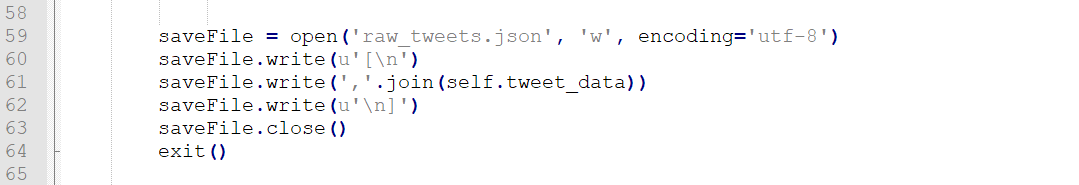
\includegraphics[width=200mm]{code51.png}
	\caption{Storing data. \label{overflow}}
\end{figure}

As shown in Figure 3-5, the block of code opens an output file, writes the opening square bracket, writes the JSON data as text separated by commas, then inserts a closing square bracket, and closes the document. This is the standard JSON format with each Twitter object acting as an element in a JavaScript array. If this is brought into the Python built-in parser, the JSON library can properly handle it.

This section can be modified to or modify the JSON file. For example, other properties/fields like a UNIX time stamp or a random variable can be placed into the JSON format. Additionally, the output file can also be modified to eliminate the need for a .csv file and insert the tweet directly into a MongoDB database. As it is written, this will produce a file that can be parsed by Python's JSON class.

After the child class is created , the instances can be created and then the stream listener can be started to store the information.

\subsection{Calling the Stream Listener:}

\begin{figure}[ht!]
	\centering
	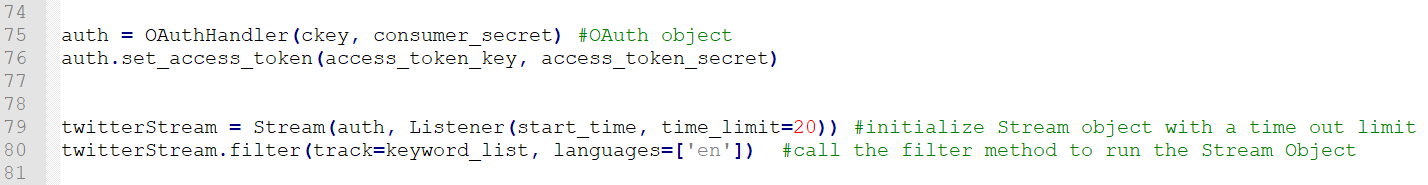
\includegraphics[width=150mm]{code61.png}
	\caption{Calling and filtering tweets in real time. \label{overflow}}
\end{figure}

As shown in Figure 3-6, the OAuthHandler uses the generated API keys [consumer key and consumer secret key] to create the auth object. The access token, which is unique to an individual user [not an application], is set in the following line. This will take all four of the credentials from the Twitter Dev site. The modified StreamListener class, simply called listener, is used to create a listener instance. This contains the information about what to do with the data once it comes back from the Twitter API call. Both the listener and auth instances are used to create the Stream instance which combines the authentication credentials with the instructions on what to do with the retrieved data. The Stream class also contains a method for filtering the Twitter Stream. The parameters are passed to the Stream API call.

\subsection{Twitter Streaming Output:}

Figure 3-7 depicts the output of the Twitter Streaming API, here the keywords used are earthquake, disaster, flood. The output is store to a flat .csv file. In the figure the green highlighted tweets specify the relevant output while the red highlighted tweets show the irrelevant information to this system. This can be parsed by passing the information through a cognitive filtering system.

\begin{figure}[ht!]
	\centering
	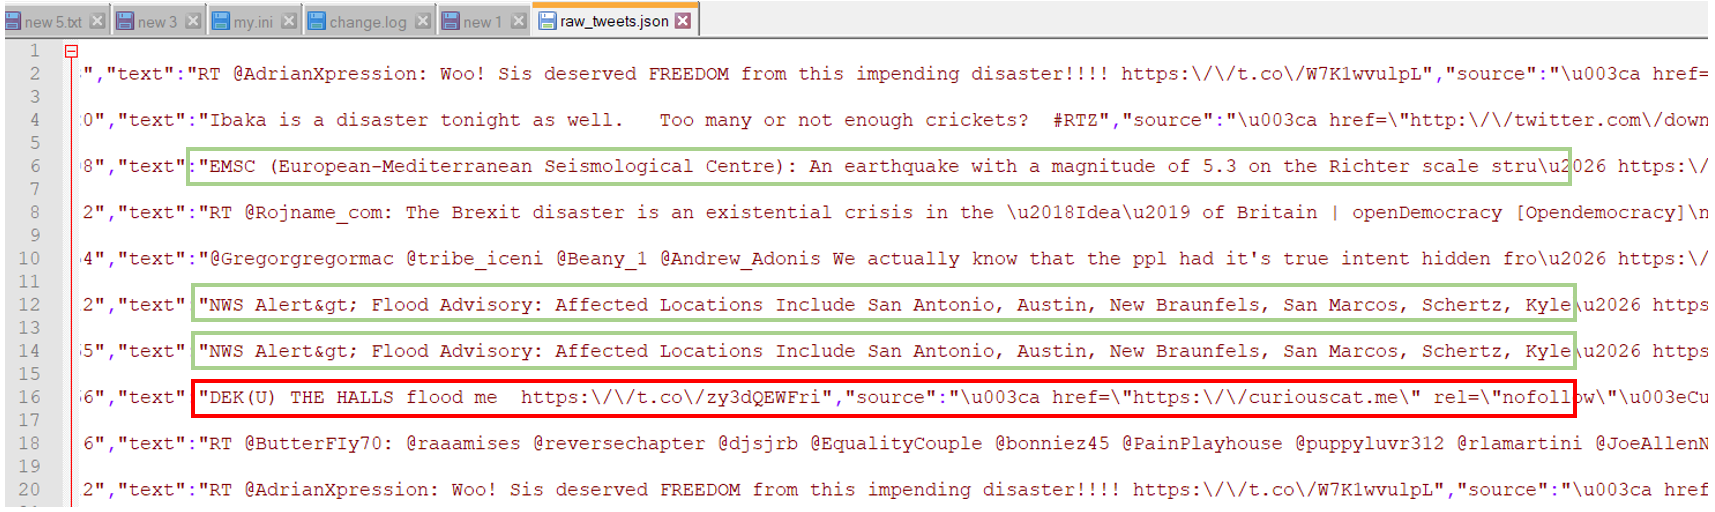
\includegraphics[width=153mm]{tweetoutput.png}
	\caption{Tweet stream output. \label{overflow}}
\end{figure}

\section{MongoDB}

Storing JSON tweets as a .csv file works well, but they don't always make good flat .csv files as not every tweet has the same structure nor do every tweet contain the same fields. Some data is well nested into the JSON objects. It is possible to write a parser that has a field for each possible subfield, but this can take a lot of time as involves a lot of considerations and will also create a large .csv file or SQL database.

NoSQL databases like MongoDB works very well as a simple tweet storage, search and recall, which eliminates the need to use an extensive tweet parser.

\subsection{What is MongoDB?}

It is a document-based database that stores data using documents rather than using tuples in tables like traditional relational databases. These documents are similar in structure to JSON objects using key-value pairs and are called BSON (Binary JSON). JSON and BSON have similar properties as JS objects and Python dictionaries.

\subsection{Why store in MongoDB?}

Storing tweets in MongoDB makes sense as BSON and JSON are so similar and that makes putting the entire content of a tweet's JSON string into an insert statement and executing that statement to store the data. This also makes recalling and searching for tweets simple although it does require a change in thought process of rather executing traditional SQL commands to treating data as OOP structures.

\section{Storing Tweets in MongoDB}

\begin{figure}[ht!]
	\centering
	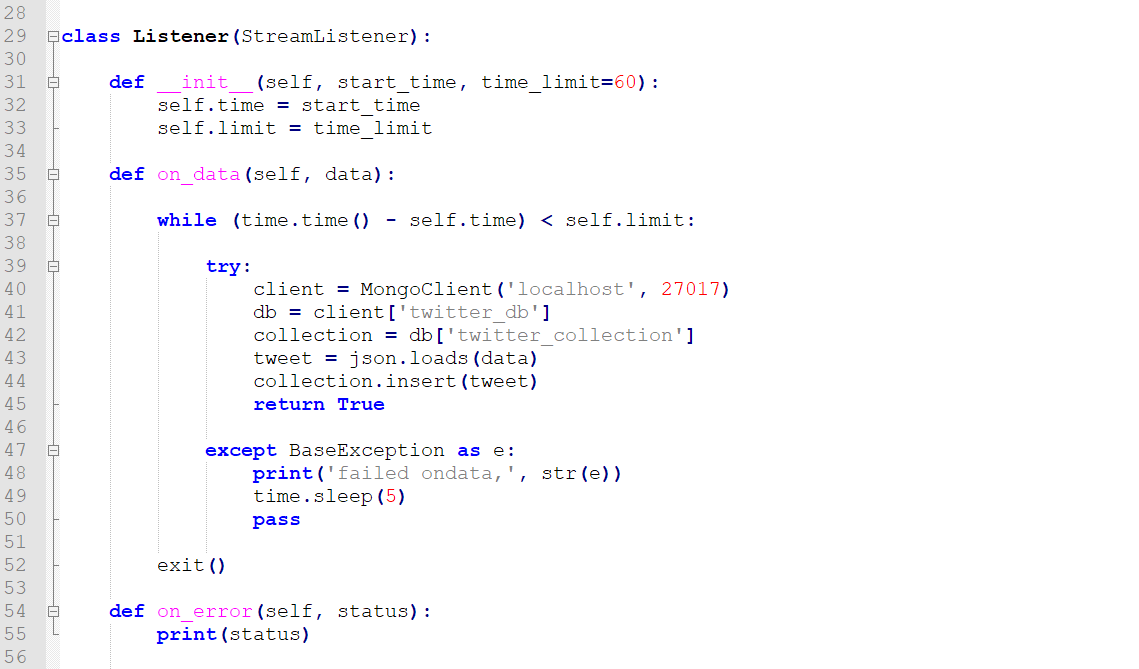
\includegraphics[width=200mm]{code71.png}
	\caption{Storing tweets in MongoDB. \label{overflow}}
\end{figure}

Once MongoDB is installed and configured storing tweets is simple using the Python stream listener. Modifying the code shown above the pymongo and JSON libraries can be imported. The JSON library is the default python library and will be available to import, pymongo needs to be set up using the following command:

\begin{lstlisting}
\$ pip install pymongo
\end{lstlisting}

The main changes in the code that was done is in the listener child class as shown in Figure 3-7.

as  shown in Figure 3-8, MongoClient creates the MongoClient instance which interfaces with the database. The client['twitter\_db'] call designates the database that is going to be used, and the db['twitter\_collection'] call selects the collection where the documents will be stored. The json.loads() call converts the string returned from the Twitter API into a JSON object in Python. Finally, the collection.insert() call inserts the JSON object into the MongoDB database. From this rather simple change to the Python stream listener all the tweets can be saved into a MongoDB database.

\section{Recalling Tweets from MongoDB}

The function to retrieve any document from a MongoDB database is collection.find(). Here, I can specify what I want or leave it black to get all the documents returned, in my case it will be all the tweets.

Calling using the .find() method, Python returns a MongoDB cursor, which can be iterated through by putting it in a for loop. The for loop will run the loop for each object in the iterator. 

\section{Context based filtering}

Context-based filtering, also referred to as cognitive filtering, recommends elements based on a comparison between the content of the elements and the requirement of the output. Content of each element is represented as a set of descriptors or terms, typically a set of words that occur in a document or in this case in the data stored in MongoDB.

\begin{figure}[ht!]
	\centering
	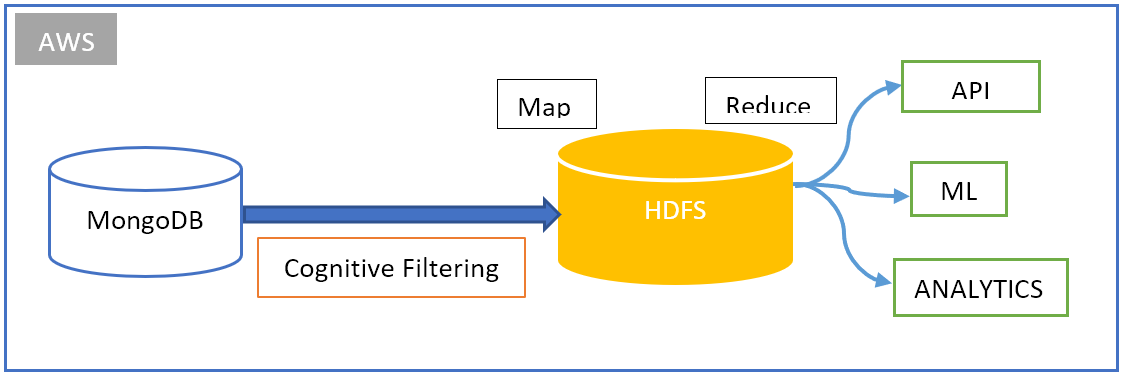
\includegraphics[width=150mm]{ContextFiltering.png}
	\caption{Cognitive filtering model. \label{overflow}}
\end{figure}

As shown in Figure 3-9, the cognitive filtering system will filter relevant information from the Streaming API output as shown in Figure 3-7. The cognitive filtering model can represent each disaster element as a set of terms that can be based on the context of the output to filter out the information.

\begin{figure}[ht!]
	\centering
	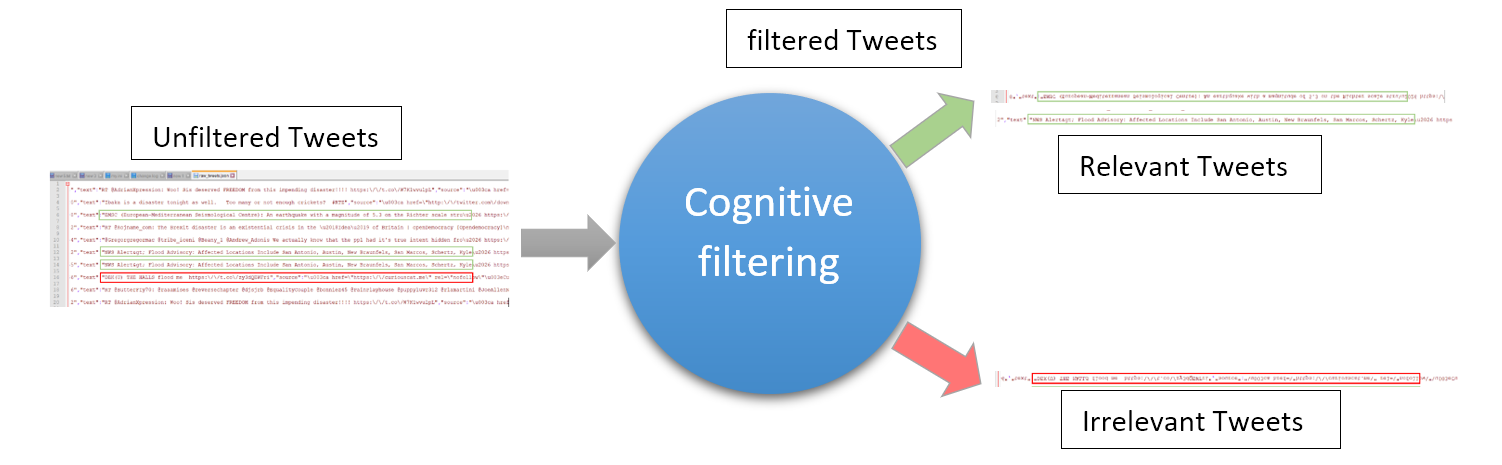
\includegraphics[width=150mm]{ContextFilteringWorking.png}
	\caption{Cognitive filtering model. \label{overflow}}
\end{figure}

As shown in Figure 3-10, the context filtering model works to filter the tweets base on relevance of the information being fed to it. The model is trained to understand the context of the data and provide output based on those requirements. With respect to filtering the disaster related data, the model takes the unfiltered data and filters the data into relevant and irrelevant information. The relevant information is sent to the Hadoop data store for further processing, the irrelevant information is discarded, saving space.

Although, it is out of scope of this research to implement a context-based filtering system, it is absolutely necessary to mention a need of a cognitive based system to filter the data before processing it, as the goal of the DMIS design is to provide a solution for fast delivery during response phase of a disaster.

\section{Hadoop}

Hadoop is a programming framework used to support the processing of large data sets in a distributed computing environment \cite{shvachko2010hadoop}. Hadoop ecosystem consists of Hadoop Kernel, Mapreduce, HDFS and number of various components like Apache Hive, Base and Zookeeper.

This study uses MapReduce framework to process the data to output the information. The framework allows processing of large dataset by using divide and conquer strategy, and run it in parallel.

The input of the Hadoop data store is the output of the context filtering model. The relevant tweets are stored in the data store. The system processes the tweets using Hadoop Map and Reduce to provide location-based information.

\section{Amazon Web Services}

Amazon Web Services (AWS), a cloud computing service, provides a platform that is ideally suited for building fault-tolerant software systems \cite{barr2011building}. As the DMIS platform aims to be operational even during a disaster, hosting it on cloud platform like AWS is a logical choice.

Amazon Elastic Compute Cloud (Amazon EC2) is a web service within AWS that provides computing resources that can be used to build and host systems. Using multiple EC2 instances, a highly reliable and fault-tolerant DMIS can be built. Also AWS provides the flexibility to scale using tools and ancillary services such as Auto Scaling and Elastic Load Balancing.

On the surface, Amazon EC2 instances behave like traditional hardware servers as they provide a virtual shell to host familiar operating systems like Linux, Windows, or Debian. Thus, providing flexibility to accommodate any type of platform to run on these systems. Additionally, a system can start small and grow when needed by adding heterogeneous nodes.

Using AWS, DMIS is poised to realize the full potential of the platform and use its services in the fullest possible way. Furthermore, gradual expansion of the system can be modular and new features can be incorporated in to the system over new nodes.

\section{Summary}

In this chapter the design of the system was described while also detailing the choices made to use certain technologies to implement the system in practice. The twitter data streaming API called the Twitter Streaming API is used and integrated in to the tweepy python library to abstract the API call for easier implementation.

The Streaming data is stored in a .csv file which is then read into MongoDB to store the information. During the streaming API call the Twitter Streaming API provides the option to extract data based on keywords. This is specified during the DMIS API call and is the first step to filter the data collected from the Twitter data store.

As the data collected is still unfiltered as it contains relevant information mixed with irrelevant information, the system has to filter this before processing it further. This is done before the data is passed to Hadoop for further processing. The unfiltered data is passed through a cognitive filtering system to sort the data based on the context of the information. The cognitive filtering model works as shown in Figure 3-10.

Once the data is filtered the relevant information is passed to the Hadoop system for processing, the Hadoop map and reduce functions are used to parse the information and structure the data that can be queried using an API call to serve different use cases. Additionally, the raw information can be provided that can be used for further analysis or parsing as needed.

All the components of the system are hosted on Amazon Web Services cloud computing platform for making it resilient to disaster related failures. In the context of this study, the system described here provides with an approach to a system that can parse disaster related data and store it continuously.